\documentclass[fontsize=12pt,paper=a4,twoside]{scrartcl}

% SWP-Präambel
% C 2003-2021 Sebastian Offermann, Rainer Koschke, Karsten Hölscher
% In Zeilen 41 und 42 sind jeweils die aktuellen Semester-Daten einzutragen.

\usepackage[utf8]{inputenc}     % Kodierung der Tex-Datei
\usepackage[T1]{fontenc}        % Korrekte Ausgabe von Sonderzeichen (Umlaute)
\usepackage[ngerman]{babel}     % Deutsche Einstellungen [ab \begin{document}]

\usepackage{bibgerm}            % Bibliographie
\usepackage{fancyhdr}           % obere Seitenränder gestalten
\usepackage{float}              % Floats Objekte mit [H] festsetzen
\usepackage{graphicx}           % Graphiken als jpg, png etc. einbinden
\usepackage{moreverb}           % zusätzliche verbatim-Umgebungen
\usepackage{pdflscape}          % PDF-Support für landscape
\usepackage[final]{pdfpages}    % Externe PDFs einbinden
\usepackage{stmaryrd}           % zusätzliche Symbole
\usepackage{supertabular}       % Tabellen über Seitenränder hinaus
\usepackage{tabularx}           % Tabellen mit vorgegebener Breite
\usepackage{url}                % setzt URLs schön mit \url{http://bla.laber.com/~mypage}

%%% Die Reihenfolge der folgenden Pakete muss beibehalten werden:
%%% varioref, hyperref, cleveref, bookmark
% Verweise innerhalb des Dokuments schick mit " ... auf Seite ... "
% automatisch versehen. Dazu \vref{labelname} benutzen
\usepackage[ngerman]{varioref}  % [vor hyperref für korrekte Verweise]
\usepackage[colorlinks=true, pdfstartview=FitV, linkcolor=blue,
            citecolor=blue, urlcolor=blue, hyperfigures=true,
            pdftex=true]{hyperref} % [vor bookmark wegen der Optionen]
\usepackage[ngerman]{cleveref}
\usepackage{bookmark}

\hyphenation{Arbeits-paket}     % Trennungsregeln

%%% Definitionen
\newcommand{\grad}{\ensuremath{^{\circ}} }
\renewcommand{\strut}{\vrule width 0pt height5mm depth2mm}
\newcommand{\gq}[1]{\glqq{}#1\grqq{}}
\newcommand{\skipInput}[1]{}

%%% Semesterkonstanten
\newcommand{\sem}{WiSe}%{SoSe}
\newcommand{\jahr}{2022/23} %2017/2018

\newif\iftoc
\tocfalse % für kleine Abgaben kein Inhaltsverzeichnis nötig
%\toctrue % für größere Abgaben mit Inhaltsverzeichnis

\newcommand{\highlight}[1]{\textcolor{blue}{\textbf{#1}}}
\newcommand{\swp}{Software-Projekt}
\newcommand{\semester}{\sem\ \jahr}

%%% Formatierungsanpassungen
% Damit Latex nicht zu lange Zeilen produziert:
\sloppy
%Uneinheitlicher unterer Seitenrand:
%\raggedbottom

% Kein Erstzeileneinzug beim Absatzanfang
% Sieht aber nur gut aus, wenn man zwischen Absätzen viel Platz einbaut
\setlength{\parindent}{0ex}

% Abstand zwischen zwei Absätzen
\setlength{\parskip}{1ex}

% Seitenränder für Korrekturen verändern
\addtolength{\evensidemargin}{-1cm}
\addtolength{\oddsidemargin}{1cm}

\bibliographystyle{gerapali}

\newcommand\documentTitle{Bitte documentTitle festlegen!}
\newcommand\groupName{Bitte groupName festlegen!}
% swpdocument verwendet die Werte von documentTitle und groupName,
% entsprechend sollten diese vorher umgesetzt werden; sonst wird eine
% Erinnerungsmeldung an der entsprechenden Stelle im Dokument platziert
% 1. Parameter: Euer/Eure Tutor:in, z. B. {Kim Harrison}
% 2. Parameter: Abgabedatum, z. B. {05. April 2063}
% 3. Parameter: Versionsnummer, z. B. {1.1}
% 4.-9. Parameter: jeweils Name und (Uni-)Email-Adresse jedes 
%                 Gruppenmitglieds; mit einem & getrennt, z. B.
% {Robin Cowl & roco@uni-bremen.de}
% Besteht die Gruppe aus weniger als 6 Personen, so werden die 
% übrigen Parameter leer gelassen: {}
\newcommand \swpdocument[8] {
% Lustige Header auf den Seiten
  \pagestyle{fancy}
  \setlength{\headheight}{70.55003pt}
  \fancyhead{}
  \fancyhead[LO,RE]{\swp{}\\%
                    \semester{}\\%
                    \documentTitle}
  \fancyhead[LE,RO]{Seite \thepage\\%
                    \slshape \leftmark\\%
                    \slshape \rightmark}

% Lustige Header nur auf dieser Seite (Titelseite)
  \thispagestyle{fancy}
  \fancyhead[LO,RE]{ }
  \fancyhead[LE,RO]{Universität Bremen\\%
                    FB 3 -- Informatik\\%
                    Tutor: #1}
  \fancyfoot[C]{}

% Start Titelseite
  \vspace{3cm}
  \begin{minipage}[H]{\textwidth}
    \begin{center}
      \bfseries \Large \swp{} -- \semester{}\\
      \smallskip
      \small 03-IBGP-SWP\\
      \vspace{3cm}
    \end{center}
  \end{minipage}
  \begin{minipage}[H]{\textwidth}
    \begin{center}
      \vspace{1cm}
      \bfseries {\Large \documentTitle}\\
      \vspace{3ex}
      $<$\groupName$>$\\%
      \vfill
    \end{center}
  \end{minipage}
  \vfill
  \begin{minipage}[H]{\textwidth}
    \begin{center}
      \sffamily
      \begin{tabular}{lr}
        #3 \\
        #4 \\
        #5 \\
        #6 \\
        #7 \\
        #8 \\
      \end{tabular}
      \\[22mm]
      \itshape Abgabe: #2\\ ~
    \end{center}
  \end{minipage}
% Ende Titelseite

\iftoc
%\iffalse
% Start Inhaltsverzeichnis
\newpage
  \thispagestyle{fancy}
  \fancyhead{}
  \fancyhead[LO,RE]{\swp{}\\%
                    \semester{}\\%
                    \documentTitle}
  \fancyhead[LE,RO]{Seite \thepage\\%
                    \slshape \leftmark\\~}
  \fancyfoot{}
  \renewcommand{\headrulewidth}{0.4pt}
\tableofcontents
% Ende Inhaltsverzeichnis
\fi

% Header für alle weiteren Seiten
\newpage
  \fancyhead[LE,RO]{Seite \thepage\\%
                    \slshape \leftmark\\%
                    \slshape \rightmark}

}


\usepackage[shortlabels]{enumitem}
\graphicspath{{./images/}}
%
% Und jetzt geht das Dokument los....
%
\begin{document}
\renewcommand\documentTitle{Datenmodell}
\renewcommand\groupName{KarteikartenAG}
\swpdocument{Rodrigue Wete Nguempnang}{20. November 2022}%
            {Mert As & meras@uni-bremen.de}%
            {Tom Beuke & tombeuke@uni-bremen.de}%
            {Efe Carkcioglu & efe1@uni-bremen.de}%
            {Nadja Cordes & ncordes@uni-bremen.de}%
            {Ole-Niklas Mahlstädt & olma@uni-bremen.de}%
            {Henry Zöllner & henry5@uni-bremen.de}%

\newcommand\cat[1]{
    \textbf{\large #1}\\[0.5em]
}

\section{Datenmodell Beschreibung}\label{sec:detailliert:Anwendungsfälle}

\cat{Card}
Eine Karte dient als abstrakte Überklasse für die unterschiedlichen Frage/Antwort Kategorien.\\
Die Grundattribute einer Karte sind die ID, das Erstelldatum sowie die Sichtbarkeit der einzelnen Karte.\\
\\
Jede Frage/Antwort Kategorie erbt die Funktionen der \texttt{Card} Klasse und enthält spezifische Frage/Antwort Attribute
je nach Art sowie Getter-/Setter-Methoden. Bei den Frageformen: ImageTest und Audio gibt es zusätzlich die Möglichkeit mit
\texttt{bSwapQA} festzulegen, dass die Frage- und Antwortoptionen getauscht werden. Es kann also eine Bild- oder Audiodatei
als Frage, als auch als Antwort verwendet werden. \\
\\
Um die Filterung über die Suchbegriffe zu ermöglichen, gibt es die Methode \texttt{getContent()}. Diese zieht aus den Fragen/Antworten mit Textinhalt die gewünschten Begriffe und wird durch die einzelnen Subklassen überschrieben. \\
\\

\cat{Tag}
Die \texttt{Tag} Klasse stellt alle aufgenommen \texttt{Tags} dar. \texttt{Tags} können auch kartenübergreifend verwendet werden.\\
Da es keine zwei \texttt{Tags} mit gleichem Namen geben soll, wird dafür \texttt{equals} in der Klasse überschrieben.\\
\\

\cat{CardToTag}
Ist eine Referenzklasse, die je \texttt{Card} und \texttt{Tag} einen Eintrag enthält und im Konstruktor übergeben bekommt.\\
Sie kann verwendet werden, um eine genaue Übersicht über die verwendeten \texttt{Tags} sowie deren zugehörigen \texttt{Cards} (und vice versa) zu bekommen.\\
Es gibt keine Setter für die Attribute \texttt{oCard} und \texttt{oTag}, da bei Änderungen neue Einträge erstellt werden.\\
\\

\newpage
\cat{Category}
Die Klasse \texttt{Category} stellt die Kategorien dar. Da diese in einer Polyhierarchie strukturiert sind, sind sowohl die \textit{Children} als auch die \textit{Parents} in der Klasse gespeichert. Wenn die Polyhierarchie bearbeitet wird, soll dies sicherstellen, dass alle zugehörigen zu bearbeitenden Kategorien schnell bearbeitet werden können. Wenn der Setter \texttt{addChild()} aufgerufen wird, wird mit Aufruf gleichzeitig das Array \texttt{aParent} des \textit{Childs} bearbeitet. Da es keine zwei Kategorien mit gleichem Namen geben soll, wird dafür \texttt{equals} in der Klasse überschrieben.\\
\\

\cat{CardToCategory}
Ist eine Referenzklasse, die je \texttt{Card} und \texttt{Category} einen Eintrag enthält und im Konstruktor übergeben bekommt. Kann verwendet werden, um eine genaue Übersicht über die verwendeten Kategorien sowie deren zugehörigen Karten (und vice versa) zu bekommen. Es gibt keine Setter für die Attribute \texttt{oCard} und \texttt{oCategory}, da bei Änderungen neue Einträge erstellt werden.\\
\\

\cat{Deck}
Das \texttt{Deck} besteht aus einer \texttt{ID}, einem zugewiesenem Namen und einer initialen \textit{Order}. Auch hier kann die Sichtbarkeit des gesamten Kastens eingestellt werden. Da es keine zwei \texttt{Decks} mit gleichem Namen geben soll, wird dafür \texttt{equals} in der Klasse überschrieben. \\
\\

\cat{CardToDeck}
Ist eine Referenzklasse, die je \texttt{Card} und \texttt{Deck} einen Eintrag enthält und im Konstruktor übergeben bekommt. Kann verwendet werden, um eine genaue Übersicht über die verwendeten \texttt{Decks} sowie deren zugehörigen Karten (und vice versa) zu bekommen. Es gibt keine Setter für die Attribute \texttt{oCard} und \texttt{oCategory}, da bei Änderungen neue Einträge erstellt werden.\\
\\

\newpage
\cat{StudySystem}
Je \texttt{Deck} gibt es auch ein \texttt{StudySystem}. Dieses ist eine abstrakte Klasse, die die Grundeigenschaften Name des Systems, Beschreibung (detaillierte Beschreibung für den Nutzer, wie das System funktioniert) und den Fortschritt je System enthält, der vom Nutzer abrufbar ist. \\
Jedes voreingestellte Lernsystem kann initiiert werden und erbt die Attribute von \texttt{StudySystem} und überschreibt diese. \\
Zudem hat jedes System einen eigenen spezifischen Zustand, wo die Karten drin gespeichert werden. Um das System zu \textit{updaten}, gibt es eine \texttt{update}-Methode. In dieser werden das Attribut Fortschritt und auch der spezifische Zustand des Systems gesetzt, daher gibt es für beide keine Setter.\\
\\

\cat{User}
Der Nutzer erstellt die Karten, Kategorien und Decks. Neben seiner \texttt{ID} hat er einen Namen sowie ein Passwort. Zudem hat er die Attribute \texttt{PassHash} und \texttt{bAuthenticated}; diese dienen dazu, dass sich der Nutzer beim Server anmelden kann. \\
In der Datenbank des Servers enthalten die Karten, Kategorien und Decks die User \texttt{ID} als Fremdschlüssel. Hiermit werden die entsprechenden Einträge je Nutzer gefiltert und falls der Nutzer gelöscht wird können sie auch entfernt werden.\\
\\

\cat{Settings}
Jeder \texttt{User} hat eigene Einstellungen. Seine Spracheinstellung, seinen Anzeigemodus, ServerAdresse und ServerPort werden darüber gespeichert.
Zudem wird die Klasse \texttt{Settings} nur einmal initiiert, daher ist sie static und hat das Attribut \texttt{SettingsInstance} \textit{(Singleton)}.

\begin{landscape}
    \thispagestyle{empty}
    %\import{images/}{Datenmodell.pdf_tex}
    %\input{datenmodell.pdf_tex}
    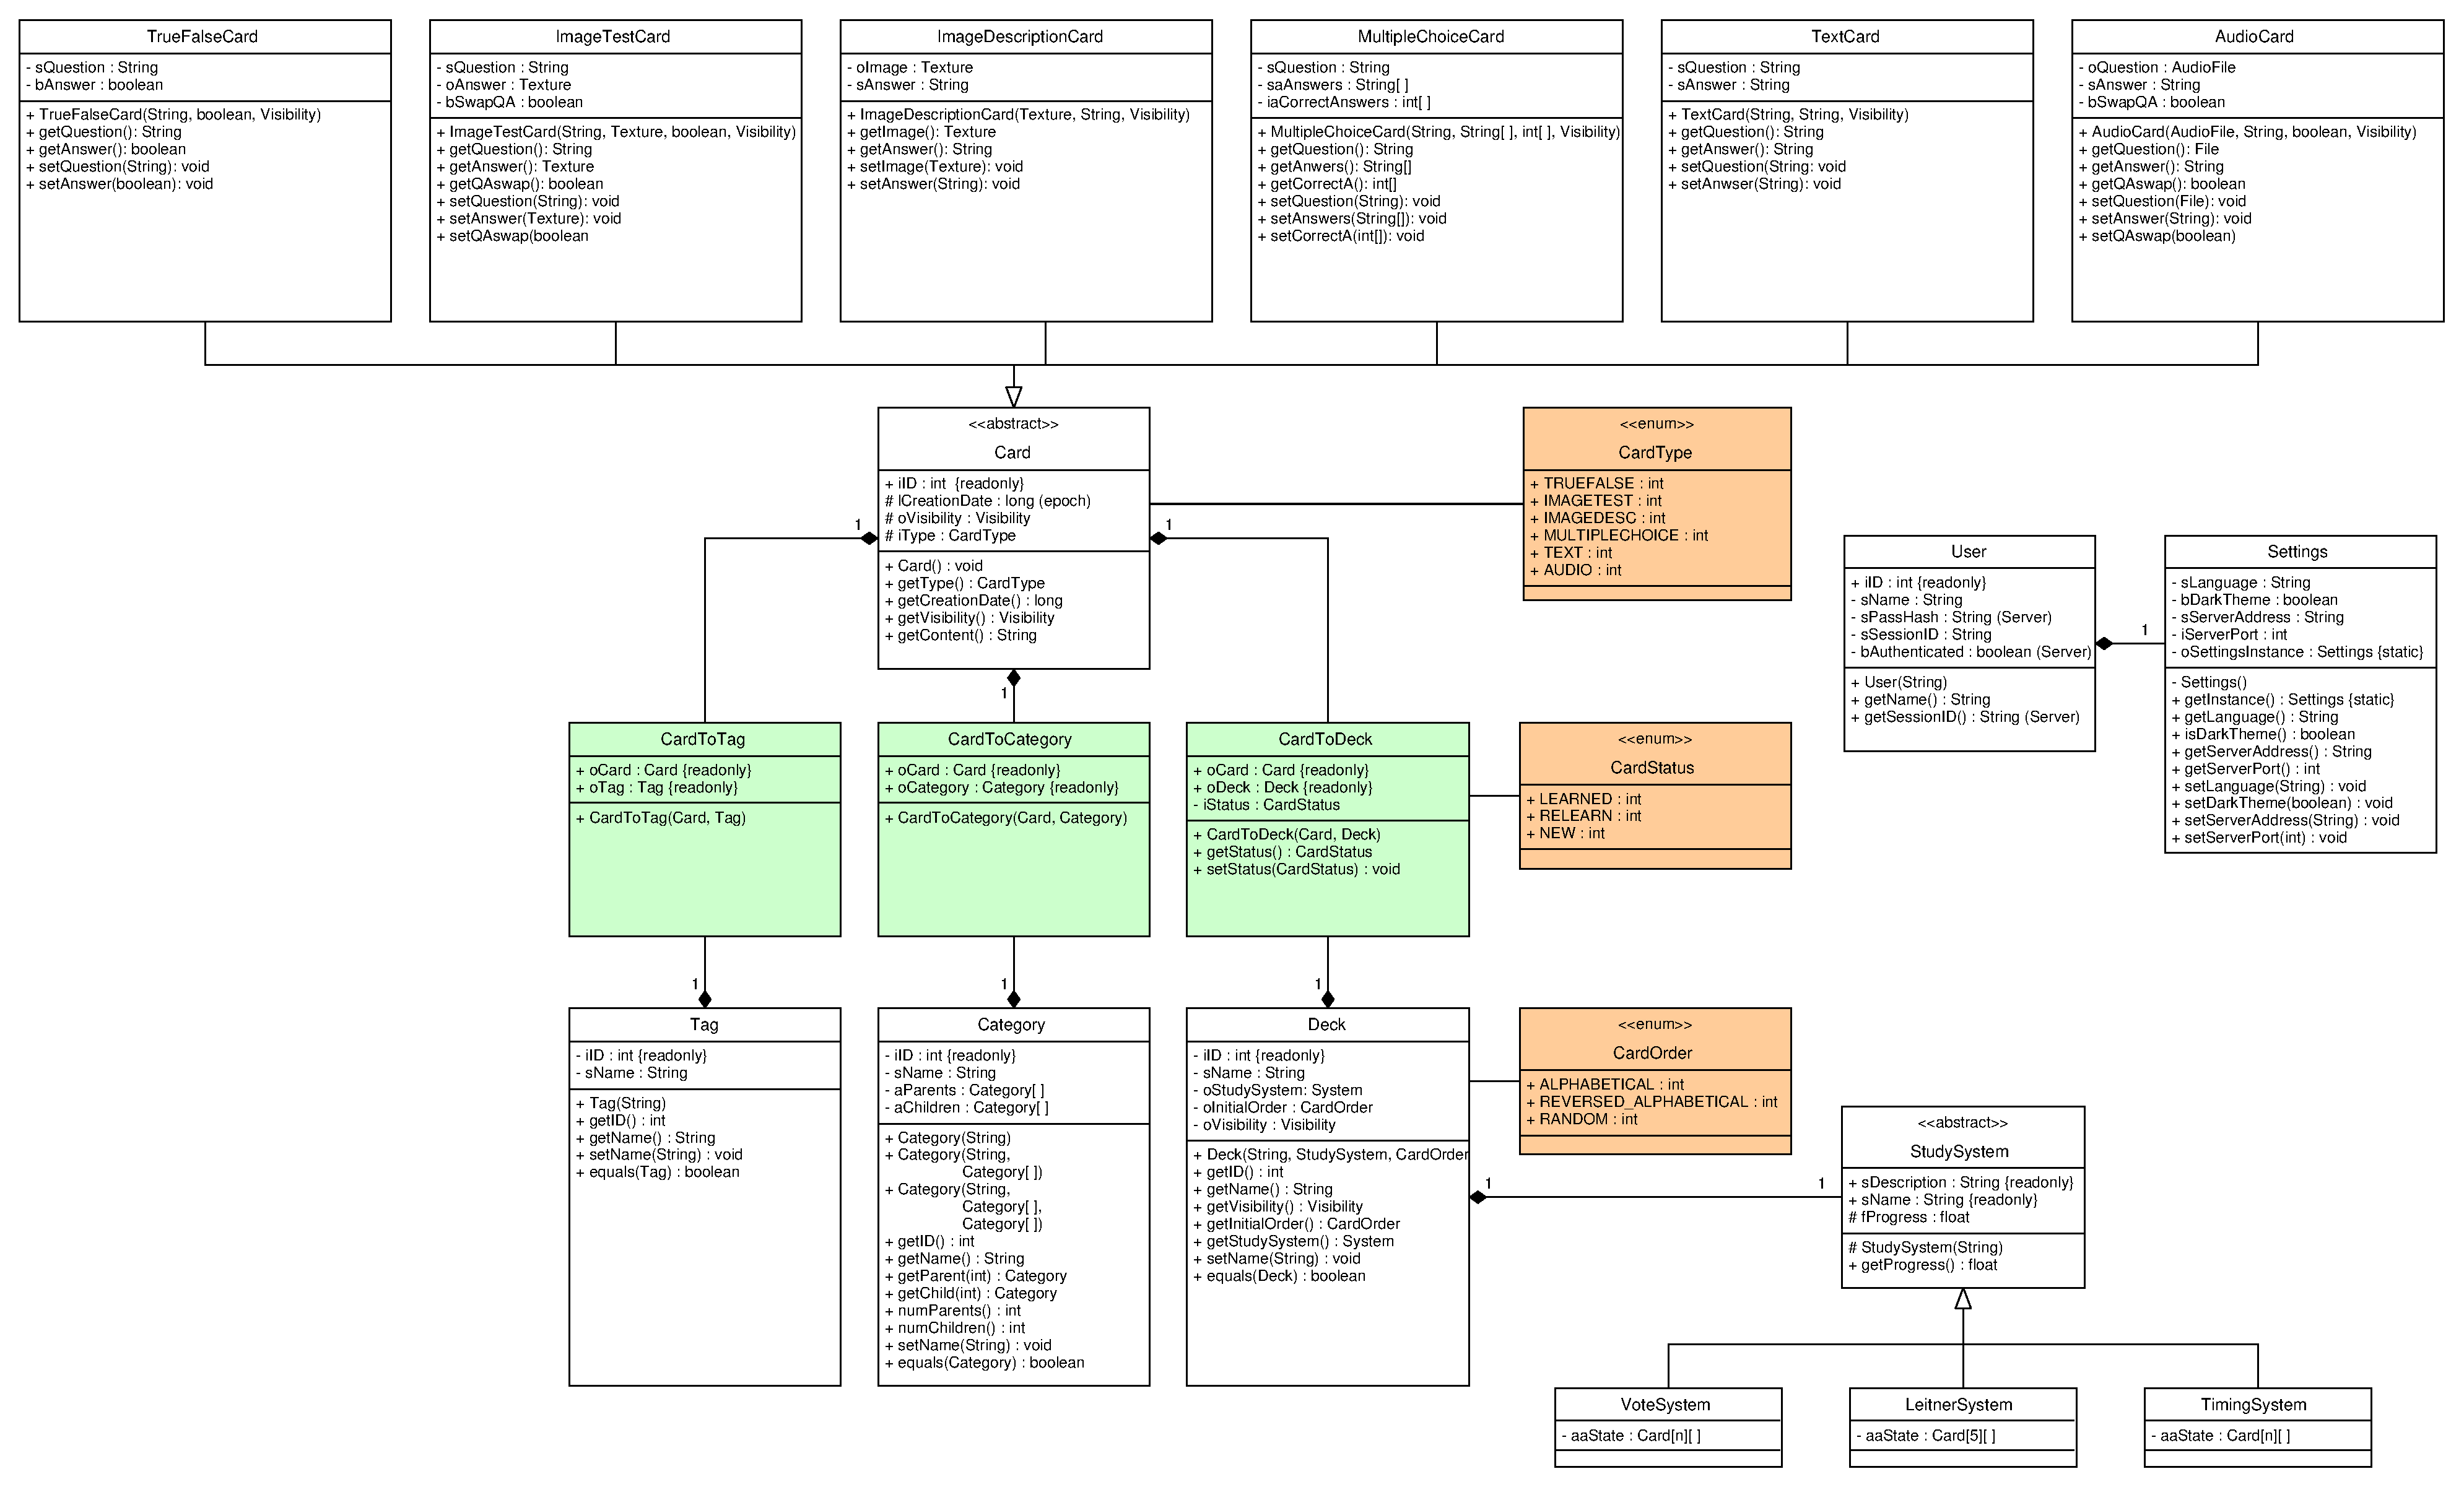
\includepdf[pages={1},angle=90]{images/datenmodell.pdf}
    %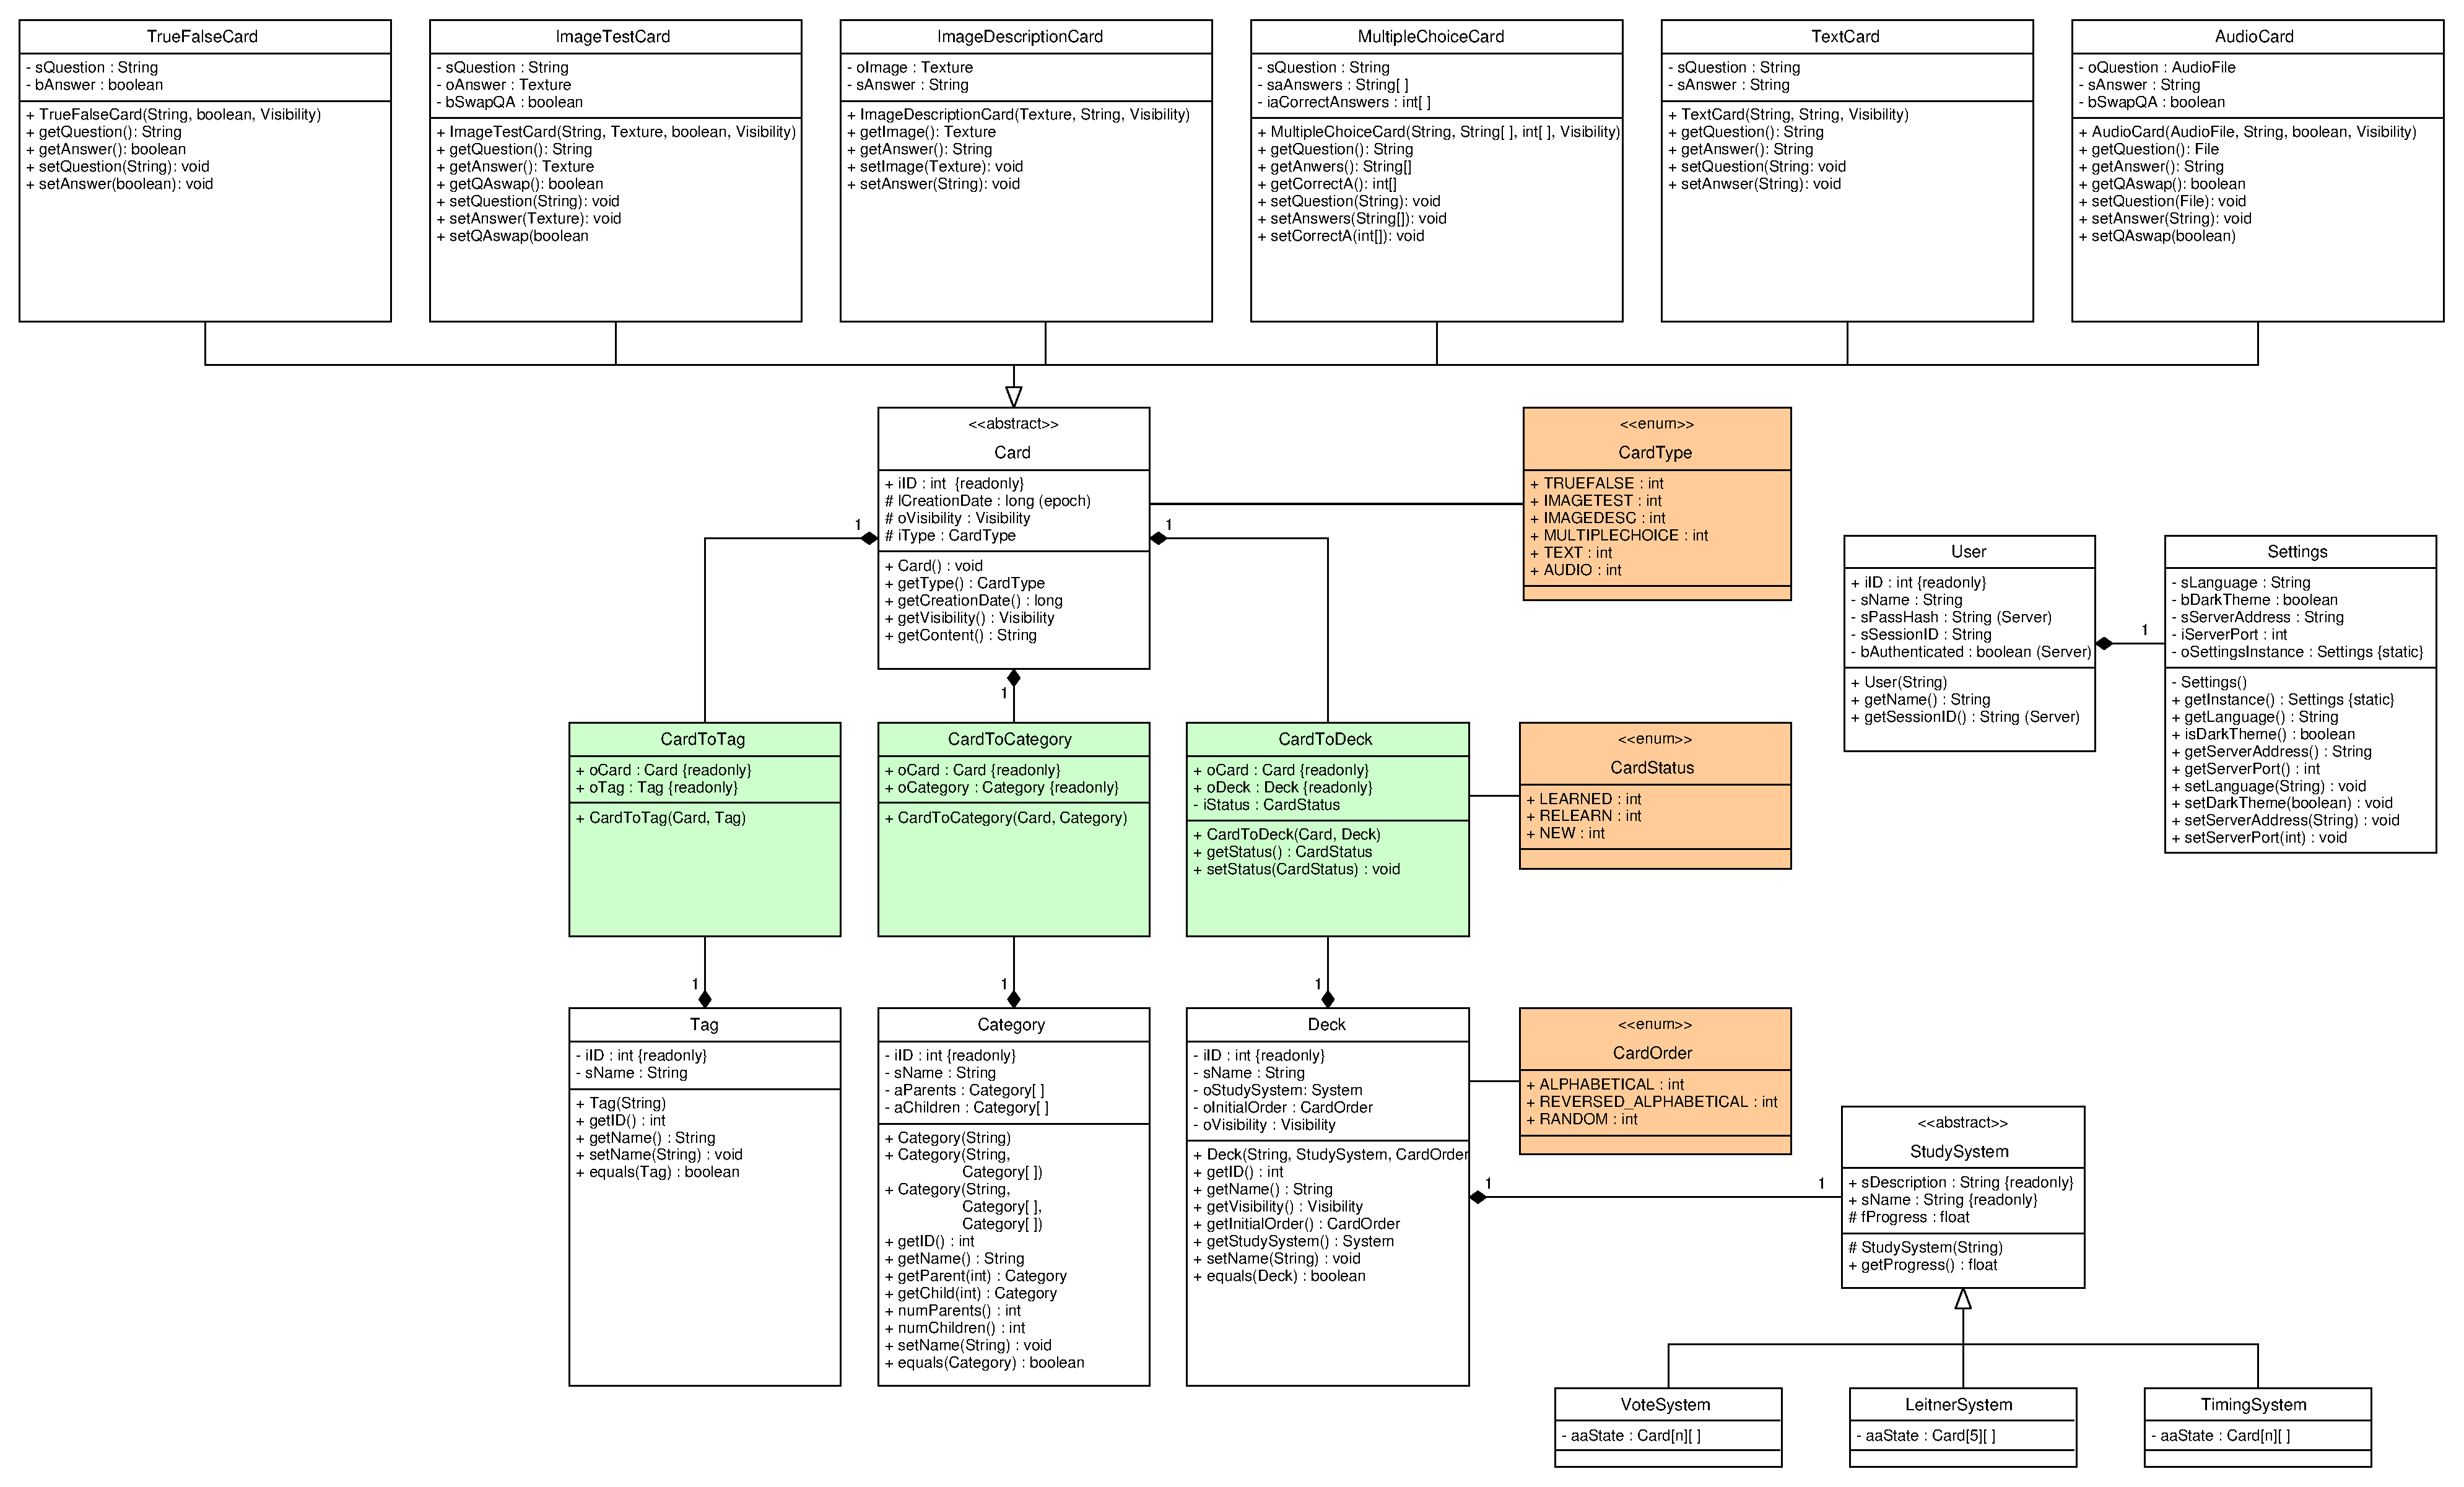
\includegraphics[scale=0.1]{images/datenmodell}
\end{landscape}

\end{document}